% Exemplo de certificados para eventos ou congressos
%
% Recomendo a leitura do manual do pacotes 'csvtools'
%
% Autor: Jes�s P. Mena-Chalco <jmena@vision.ime.usp.br>
% Wed Jul 14 17:20:29 BRT 2010

\documentclass{article}
\usepackage[brazil]{babel}
%\usepackage[latin1]{inputenc}

%\usepackage[brazilian]{babel}
\usepackage[utf8]{inputenc}
\usepackage[T1]{fontenc}

\usepackage[pdftex]{graphicx}   
\usepackage{xspace}
\usepackage{csvtools}
\usepackage{tikz}
\setcsvseparator{;}
\renewcommand{\trim}[1]{}



\usepackage{fancyhdr}
\usepackage[usenames,svgnames,dvipsnames,table]{xcolor}
\usepackage[none]{hyphenat} 
\usepackage{setspace}
\usepackage[vcentering,landscape,a4paper,
            top=1.54cm,bottom=2.54cm,
            left=1.54cm,right=1.54cm]{geometry}


\usepackage{transparent}
\usepackage{eso-pic}



\definecolor{cadet}{rgb}{0.33, 0.41, 0.47}
\definecolor{coolblack}{rgb}{0.0, 0.18, 0.39}
\definecolor{darkmidnightblue}{rgb}{0.0, 0.2, 0.4}

%%% marca de �gua -- https://texblog.org/2012/02/17/watermarks-draft-review-approved-confidential/
%%%
%\usepackage{draftwatermark}
%\SetWatermarkText{\includegraphics[width= \textwidth]{klee_b.pdf}}
%\SetWatermarkScale{2}
%\SetWatermarkAngle{0}

%
%\usepackage{xwatermerk}
%\newwatermark[allpages]{\includegraphics[width= 4cm]{klee.jpg}}
%

% Defini��es para o fancyhdr
\lhead{}
\chead{ }
\rhead{}
\renewcommand{\headrule}{\color{white}}

\cfoot{
\begin{minipage}{0.957\textwidth}
\begin{tabular}{p{\textwidth}}
  \cellcolor{cadet}  \\  
  \cellcolor{cadet}  
    \textcolor{white}{\Large{\textbf{University of Porto,  Portugal -- 1-3 Oct 2025}}} 
\\
      \cellcolor{cadet}  
\end{tabular}
\end{minipage}
}

%\cfoot{\includegraphics[width=\textwidth]{imagens/footer.jpg}}


\pagestyle{fancy}



\newcommand\BackgroundPic{%
  %\put(35,300){%
  
  \parbox[b][\paperheight]{\paperwidth}{%
    \vfill
    \centering
      \vspace{2cm}
    {\transparent{0.24} 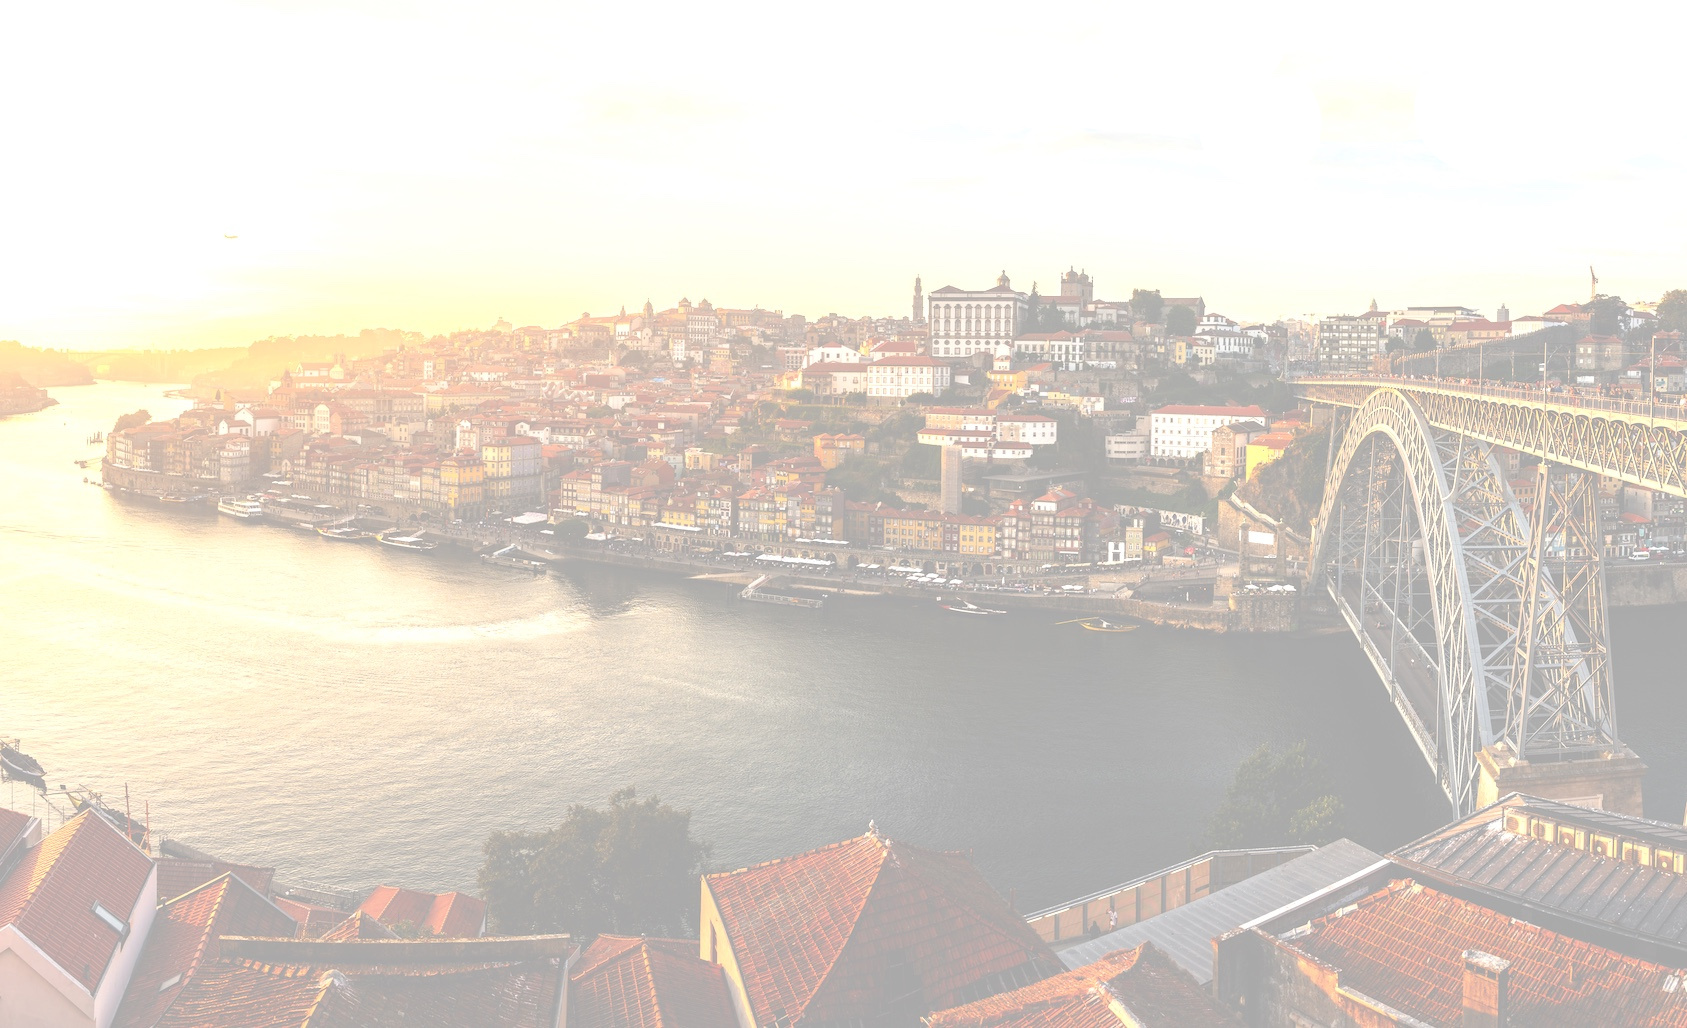
\includegraphics[scale=0.53]{apm-bg.jpg}}%
    \vfill
}}%}



%..and put this immediately after \begin{document}:

\AddToShipoutPicture{\BackgroundPic} %Compilar duas vezes para aparecer em background

%\AddToBackground{1}{%  Background of a small page
%  \put(0,0){\transparent{0.8} \textcolor{YellowOrange}{\rule{\paperwidth}{\paperheight}}}}

\AddToShipoutPicture*{ \put(0,0){\textcolor{YellowOrange}{\rule{\paperwidth}{\paperheight}}}}




% Documento
\begin{document}
  % \applyCSVfile{../SEFMv2.csv}
  % \applyCSVfile{../cifma.csv}
  % \applyCSVfile{../ibex.csv}
  \applyCSVfile{responses.csv}
  % \applyCSVfile{../reacts.csv}
  {
    \doublespacing
    \noindent    
    
    \begin{minipage}{0.957\textwidth}
      \begin{tabular}[c]{p{\textwidth}}
        %  \cellcolor{black}  \\  
        %  \cellcolor{black}  
        \cellcolor{cadet}
        \begin{center}\textcolor{white}{\Huge{\textbf{APM 2025}}}\\[-1mm]~\end{center}
        \\
            \end{tabular}
          \sffamily
      \bigskip
      \bigskip
      
      \begin{center}
        \vspace{0.5cm}
        \textcolor{darkmidnightblue}{\Huge \textbf{Certificate}}\\
        \bigskip
        \bigskip
      \end{center}
      
      \begin{center}
        \textcolor{darkmidnightblue}{    
        \begin{minipage}{0.8\textwidth}
          {\LARGE This is to certify that {\bf \insertName}\ participated in the 
7th International Workshop on
Asynchronous Programming Models (APM 2025), on 1-3 October 2025 at the
            \texttt{University of Porto}\insertIntro\emph{\insertPresentation}.
            % talk \ \emph{\insertTalk}.
          }
      \end{minipage} }
    \end{center}
    
    \vspace{2.0cm}
    \singlespacing 
  
    \begin{tikzpicture}[remember picture,overlay]
     \node[align=center,yshift=-25mm] at (current page.center)%
       {\includegraphics[width=30mm]{signature.png}};
    \end{tikzpicture}  

    \begin{tikzpicture}[remember picture,overlay]
     \node[align=center,yshift=-40mm] at (current page.center) {
         \textcolor{darkmidnightblue}{ \LARGE \rule{7.0cm}{0.5pt}}
        \\[3mm]
         \textcolor{darkmidnightblue}{\LARGE José Proença}
        \\[1mm]
         \textcolor{darkmidnightblue}{\LARGE (On behalf of the organization of APM 2025)}
     };
     \node[anchor=south east, yshift=27mm,xshift=-18mm]
         at (current page.south east) {
\includegraphics[width=20mm]{logo.png}};
     % \node at ([xshift=-2cm,yshift=1cm]current page.south east)       {\includegraphics[width=15cm]{example-image-duck}};  
    \end{tikzpicture}  


    % \textcolor{darkmidnightblue}{\begin{center}
    %     \LARGE {\rule{7.0cm}{0.5pt}\\
    %     {José Proença\\ %\insertOrganisers yields an error (the last column always)
    %       (On behalf of the organization of APM 2025)\\}}
    % \end{center}}
    
  \end{minipage}
}
\end{document}
